\documentclass{article}

\usepackage{graphicx}
\usepackage{hyperref}
\usepackage{tabularx}

\title{Project: Movie Recommendation Engine}
\author{Karsten Poddig}

\begin{document}

\maketitle

\begin{abstract}
The project described in this report is a Movie Recommendation Engine\\

\textbf{Github Repo:} \url{https://github.com/KarstenPoddig/django_movie_project}\\

\textbf{Keywords:} Data Science, Data Engineering, Statistical Dashboard, Analytics, Movie Recommendation Engine, Hierarchical Clustering,  Python, Django, Docker, Kubernetes, Continious Integration, Continious Development, Google Cloud Platform, SQL, PostgreSQL, JavaScript, Git, GitHub


\includegraphics[scale=0.055]{logos/python_logo.png}
\hspace{5mm}

\includegraphics[scale=0.1]{logos/scikit_learn_logo.png}
\hspace{5mm}

\includegraphics[scale=0.04]{logos/django_logo.png}
\hspace{5mm}

\includegraphics[scale=0.035]{logos/postgresql_logo.png}
\hspace{5mm}

\includegraphics[scale=0.12]{logos/docker_logo.png}
\hspace{5mm}

\includegraphics[scale=0.08]{logos/kubernetes_logo.png}
\hspace{5mm}

\includegraphics[scale=0.015]{logos/gcp_logo.png}
\hspace{5mm}

\includegraphics[scale=0.15]{logos/js_logo.png}
\hspace{5mm}
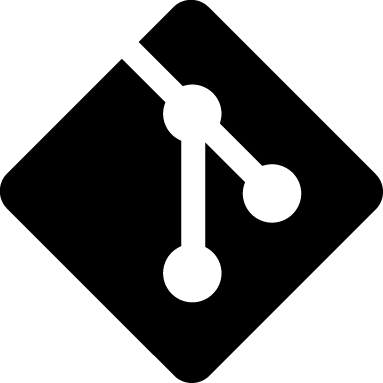
\includegraphics[scale=0.05]{logos/git_logo.png}
\hspace{5mm}

\includegraphics[scale=0.04]{logos/github_logo.png}

\end{abstract}

\tableofcontents

\newpage


% #################### Introduction #######################################
\section{Introduction}






% #################### Usage of App #######################################
\section{App functionalities}

This section provides a quick overview of the functionalities of this app. The following functionalities can be accessed without an account:

\begin{itemize}
	\item Search Movies
	\item Search for similar movies for a specific movie
\end{itemize}
The main functionalities require an account. These functionalities include

\begin{itemize}
	\item Rate Movies
	\item Get Suggestions based on your ratings
\end{itemize}
Since the main purpose of this project is to provide movie suggestions I recommend to sign in if you want to explore this app. You can do this by creating an account and create your own ratings. But rating a sufficient number of movies can be time consuming, so if you want to go on fast and simply want to explore what how this app works you can simply use the following account with exisiting ratings:\\

\begin{tabular}{|l|l|}
\hline
username & testuser \\
\hline password & password\\
\hline
\end{tabular}\\

The following subsections guide you through the app. But since the app should be somehow intuitive you can also skip these subsections.

\subsection{Sign up / Sign In}

\subsubsection*{Sign Up}

Click on the button in the right top corner and enter all necessary data.\\[2ex]
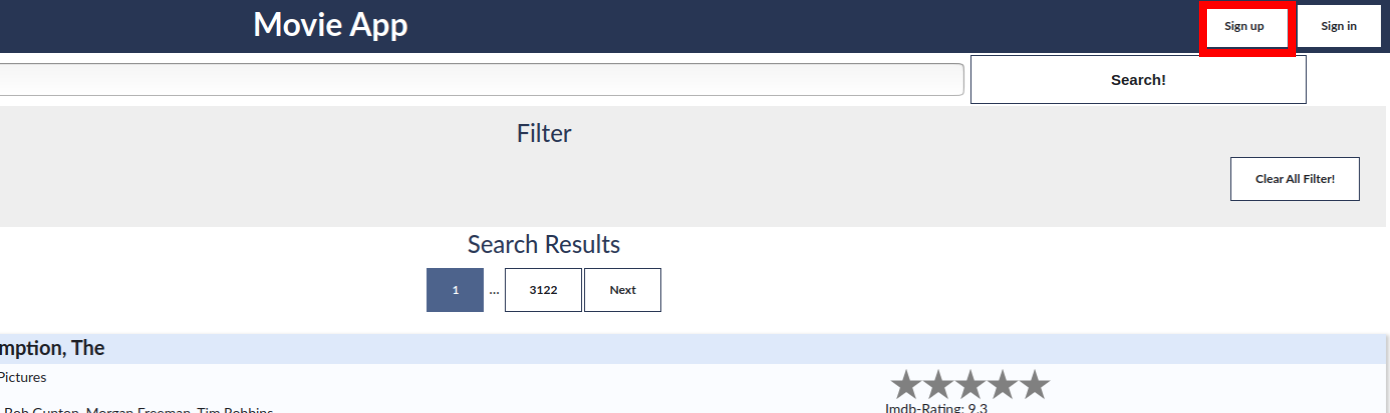
\includegraphics[scale=0.3]{screenshots_app/sign_up.png}\\

\subsubsection{Sign In}

Click on the button in the right top corner and all necessary data.\\[2ex]
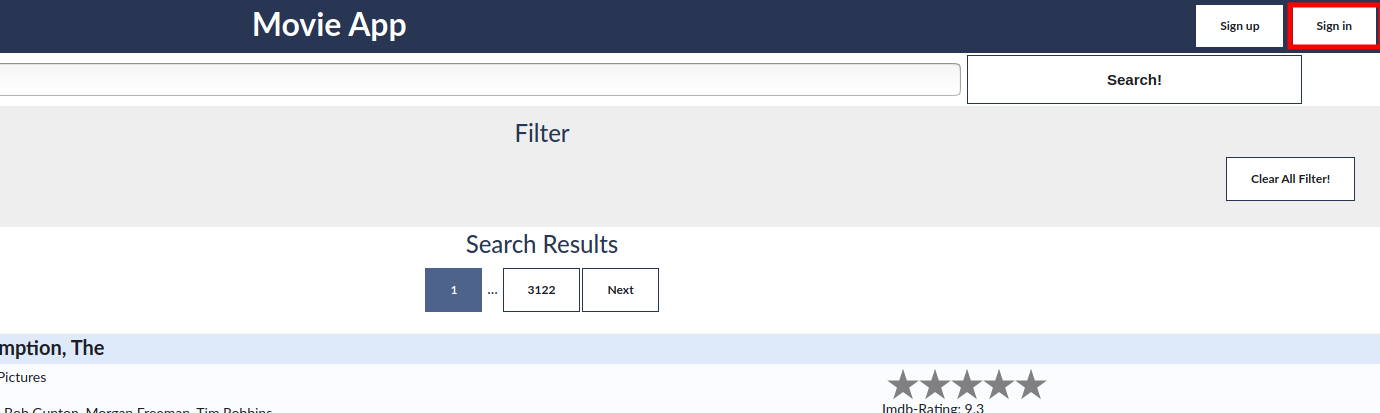
\includegraphics[scale=0.3]{screenshots_app/sign_in.png}\\
Also you are redirected to the Sign In - page if you are accessing areas which require a login (like Rated Movies, etc.)


\subsection{Search Movies}

Click on the link 'All Movies' in the left bar. You will see a list of all movies in the database with the regarding details.
To search a movie you can enter parts of title (green area) and optionally set certain filter critria (yellow area). The results are ordered decreasingly by popularity (total number of ratings).\\[2ex]
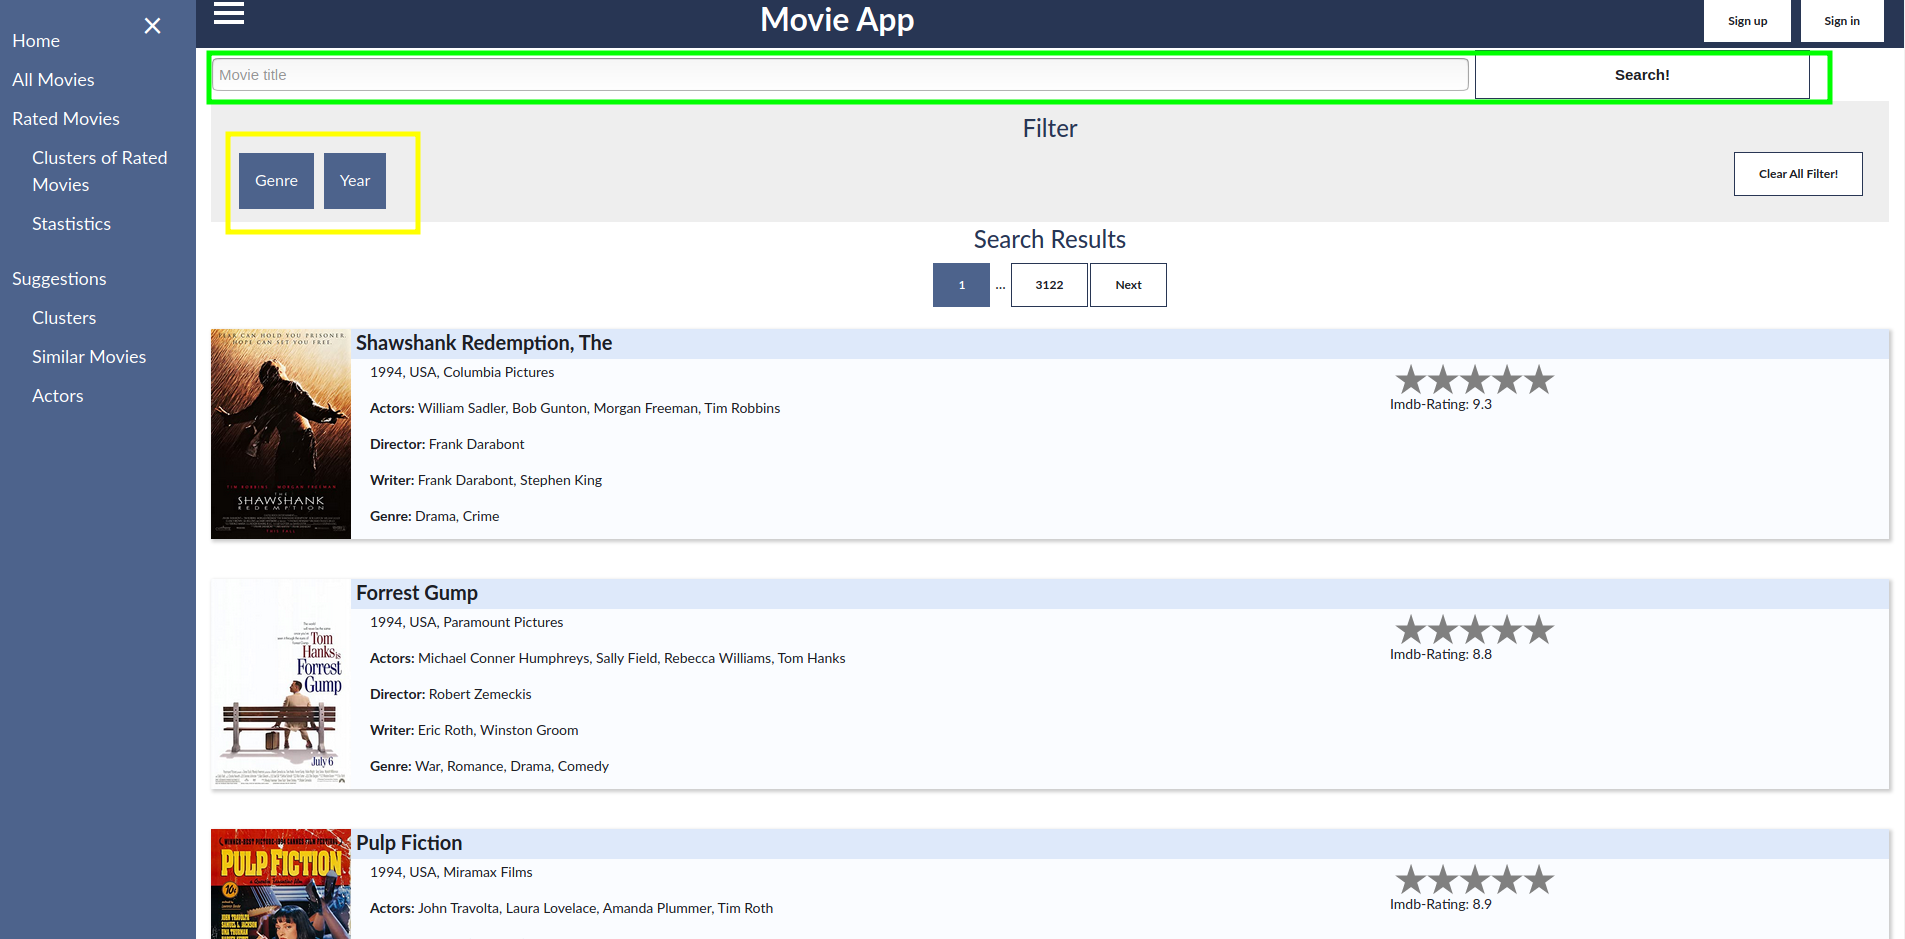
\includegraphics[scale=0.25]{screenshots_app/all_movies.png}\\

For example a search for movies with the term 'Bad' in the title with the Genre Action in the 2000s will look like the following:\\[2ex]
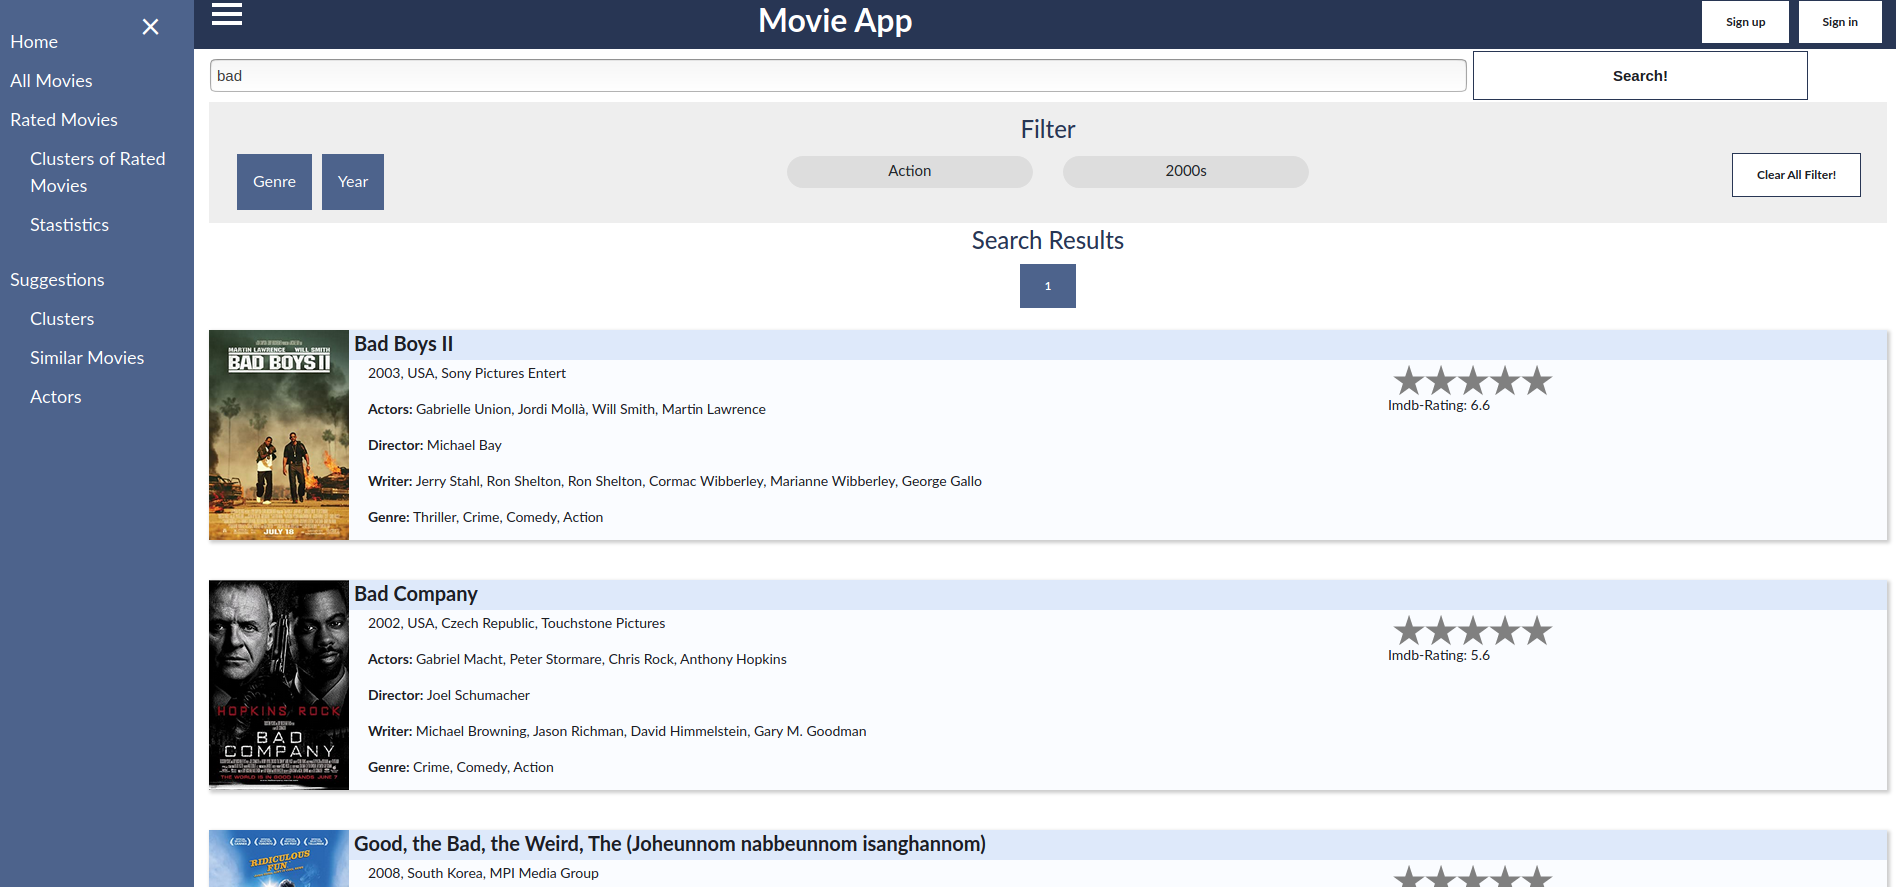
\includegraphics[scale=0.2]{screenshots_app/all_movies_ex1.png}\\


\subsection{Rate Movies}

Once you are logged in you can rate movies. Just enter the page 'All Movies', search the movie you want to rate and click on the regarding rating (red area in the following picture). If you choose a rating of 0 stars an existing rating will be deleted.\\[2ex]
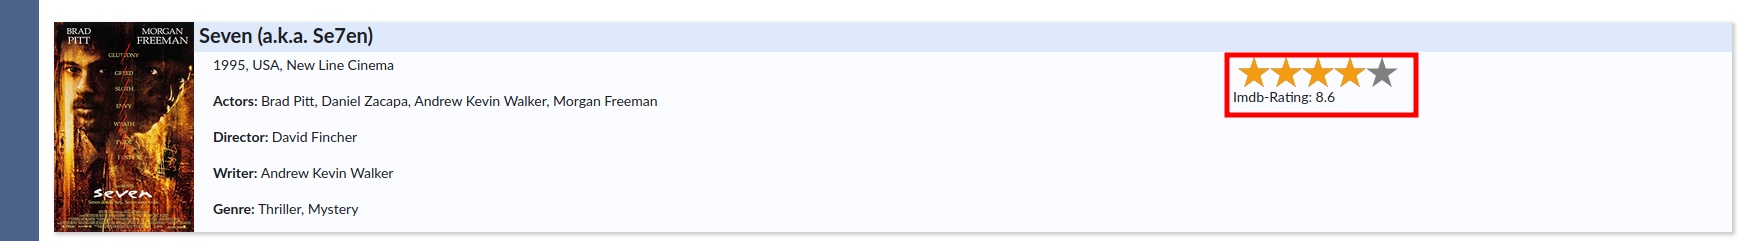
\includegraphics[scale=0.3]{screenshots_app/rate_movie_ex1.png}\\


\subsection{View Rated Movies}

At some point you maybe want to take a look at the movies you already rated. The links for the sections 2.4.1-2.4.3 are displayed in the following picture.
\\[2ex]
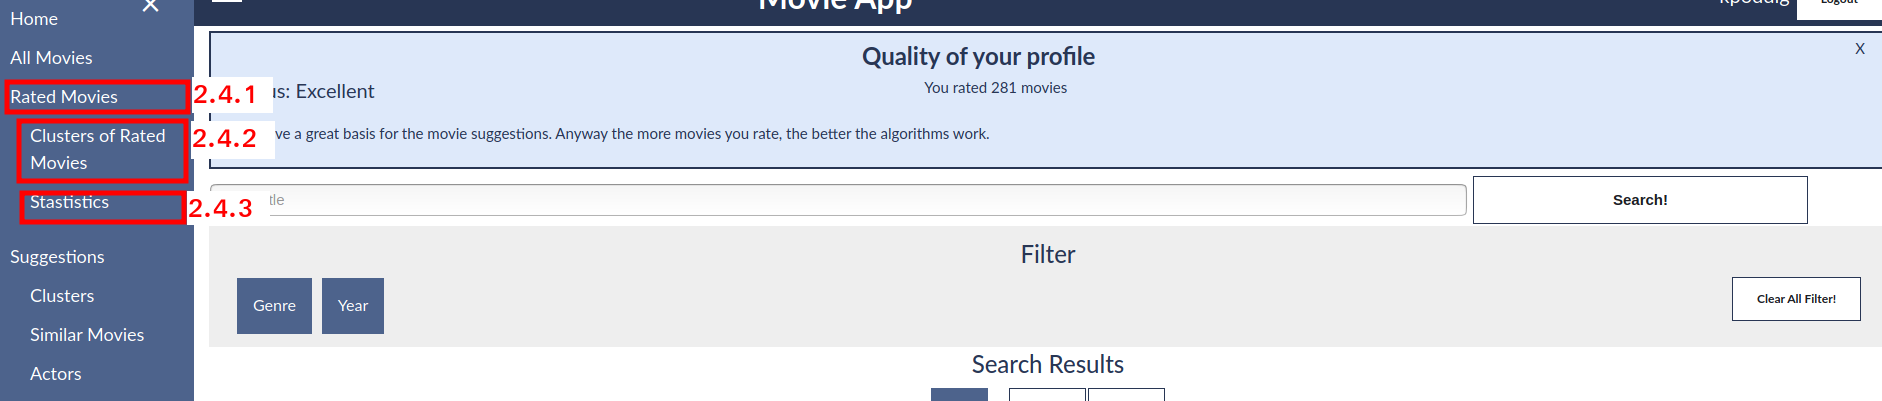
\includegraphics[scale=0.3]{screenshots_app/rated_movies_navigation.png}\\


\subsubsection{Movies with Details}

This is basically the same page as 'All Movies' (section 2.2) with the exception that just rated movies are listed here. You can search and navigate through your rated movies in the same way as in section 2.2.

\subsubsection{Clustered Movies}

To determine better suggestions your rated movies are clustered. Take a look at section. Basically each cluster (each line) contains movies which are similar to each other. Factors which imply a similarity could be the genre, the production year, the atmosphere, actors, etc. For a better understanding what similarity in this context means I again refer to Section .... .
If you want to update the clustering hit the button 'Refresh Cluster' (marked red).\\[2ex]
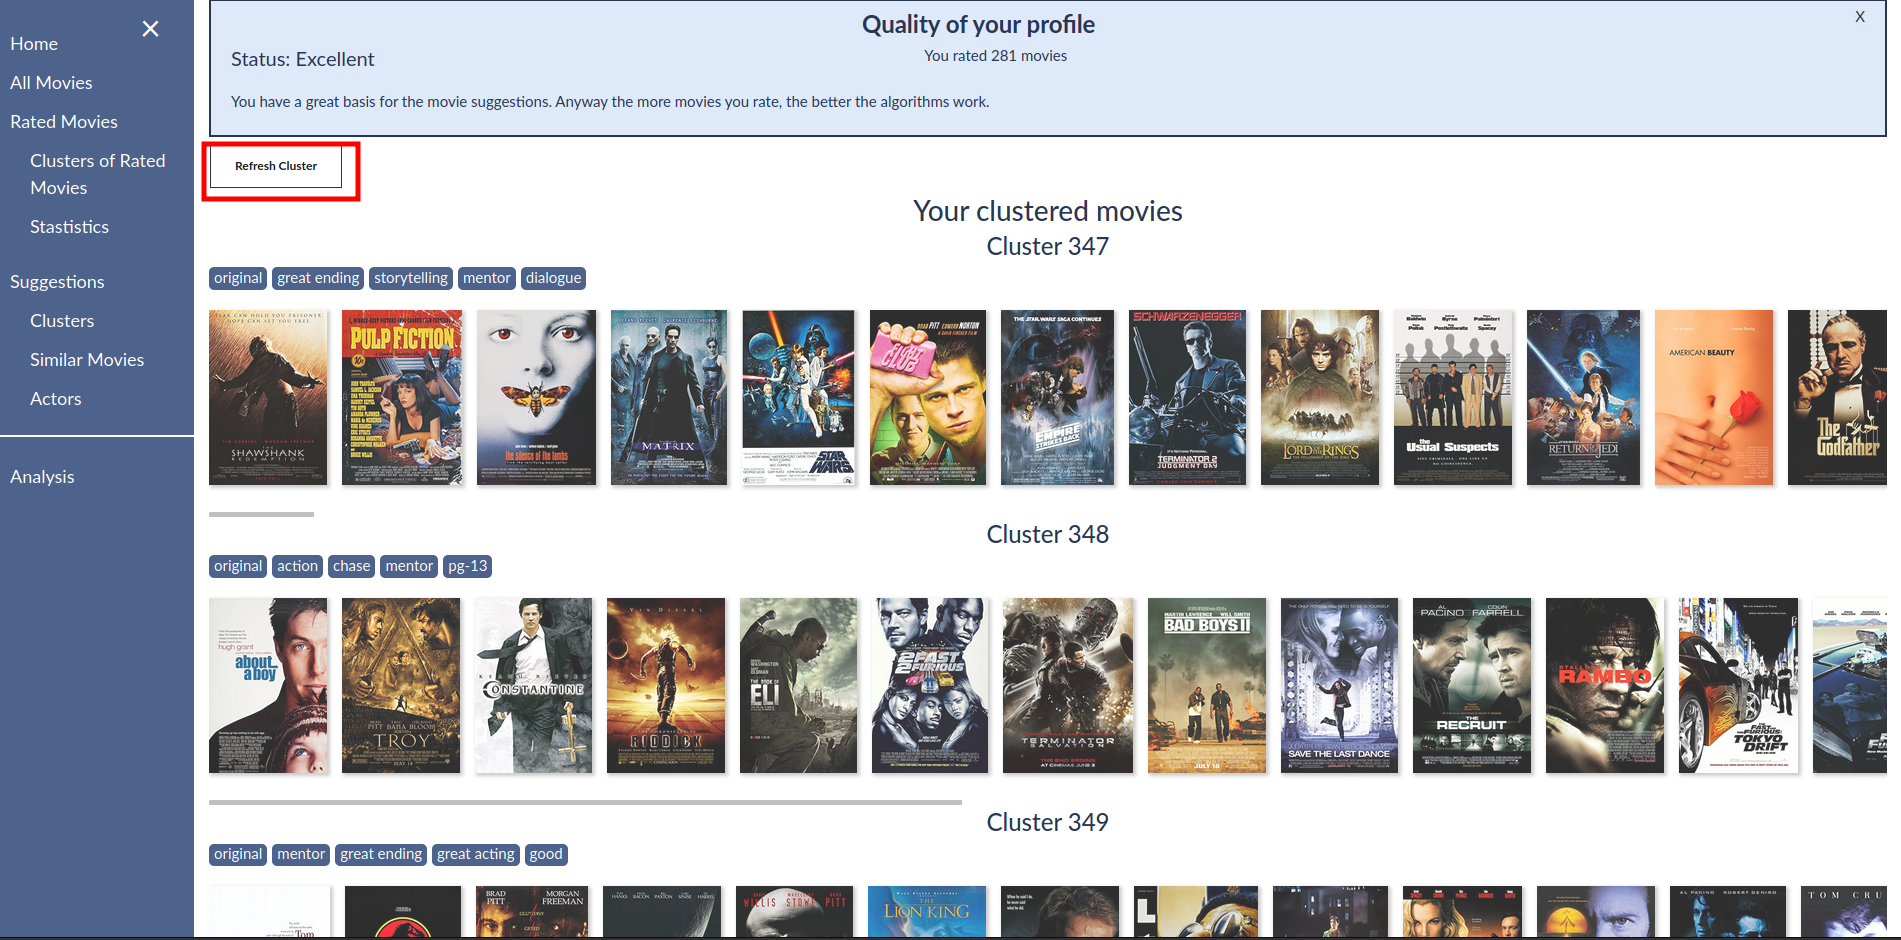
\includegraphics[scale=0.3]{screenshots_app/rated_movies_clustered.png}\\


\subsubsection{Statistics}

This page provides a statistical dashboard for your ratings.\\[2ex]
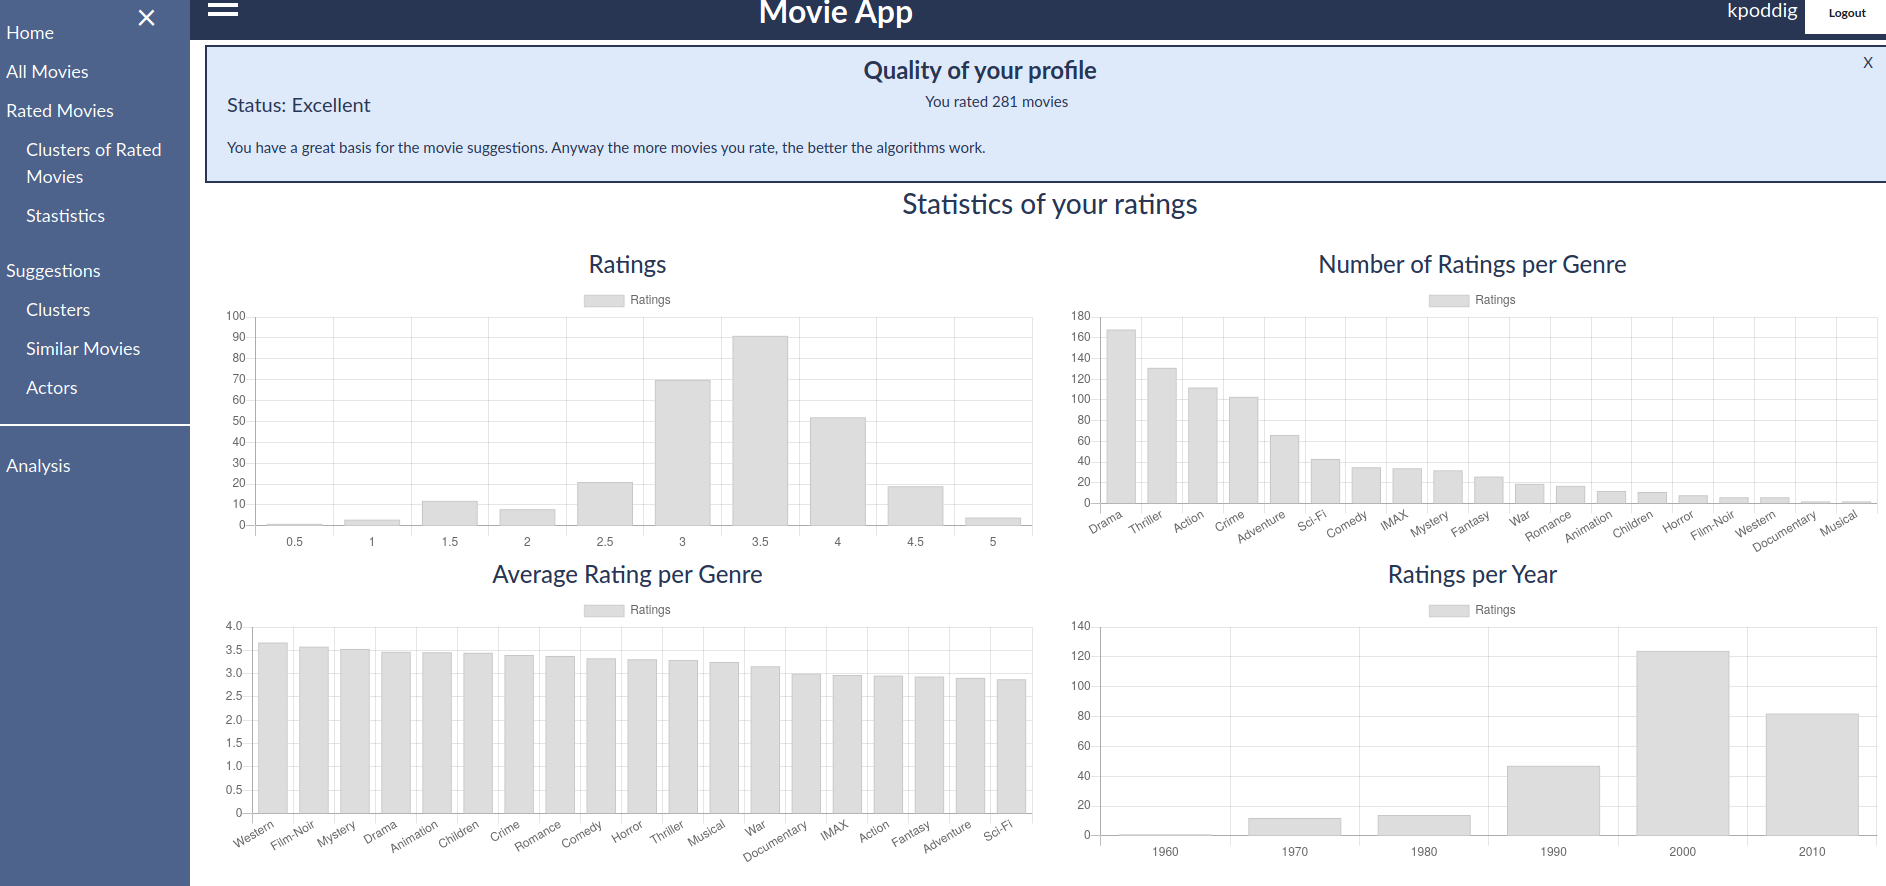
\includegraphics[scale=0.2]{screenshots_app/rated_movies_statistics.png}\\





\subsection{View Suggestions}

Now it comes to the core functionality of the app. The following picture displays the links to the sections 2.5.1 - 2.5.3.

\subsubsection{Suggestions based on clusters}



\subsubsection{Search Similar Movies}



\subsubsection{Suggestions based on Actors}





% #################### Data Science Part #################################
\section{Data Science Part}

\subsection{Similarity}

\subsection{Suggestions}


% #################### Data Engineering Part #############################
\section{Data Engineering Part}

\subsection{Source of Data}

MovieLen, Imdb-API
Own ratings


\subsection{Google Cloud SQL}






\end{document}